% This document is compiled using pdfLaTeX
% You can switch XeLaTeX/pdfLaTeX/LaTeX/LuaLaTeX in Settings

\documentclass[a5paper, twoside]{article}
\usepackage{ctex}
\usepackage{csquotes} % 对于智能引用符号
\usepackage[backend=biber,style=numeric]{biblatex} % 使用biblatex和biber
\usepackage{geometry}
\usepackage{graphicx}
\usepackage{listings}
\usepackage{minted}
\usepackage{amsmath}
\usepackage{amsfonts}
\usepackage[T1]{fontenc}
\usepackage{lmodern}
\usepackage{amssymb}
\usepackage{marginnote}
\usepackage{xcolor}
\usepackage{hyperref}
\usepackage{todonotes}
\usepackage[utf8]{inputenc}
\usepackage{mdframed}
\usepackage{multicol}
\usepackage{url} % 加载url包
\usepackage[linesnumbered,ruled,vlined]{algorithm2e}
\usepackage{array} % 提供>{...}功能
\usepackage{booktabs} % 提供更好的表格线条
\usepackage{lipsum} % 用于生成占位文本
\usepackage{titlesec}
\usepackage{titling}
\usepackage{wrapfig}
\usepackage{enumitem}
\usepackage{graphicx}
\usepackage{tikz}
\usepackage{newtxmath}
\usepackage{caption}
\usepackage{fancyhdr}  % 用于设置页眉和页脚
\usepackage{tocloft}  % 用于自定义目录
\usepackage{fontspec}
\setmainfont{Times New Roman}
% 设置 hyperref 的一些选项
\hypersetup{
	colorlinks=true,  % 使用颜色而不是框
	linkcolor=myblue,   % 内部链接的颜色
	urlcolor=cyan,    % URL 链接的颜色
	citecolor=green,  % 引用链接的颜色
	bookmarks=true,   % 创建书签
}
% 设置目录标题
\renewcommand{\contentsname}{\textbf{目录与索引}}
% 调整各级标题的缩进
\setlength{\cftsecindent}{0em}  % 小节缩进
\setlength{\cftsubsecindent}{2em}  % 子小节缩进
\setlength{\cftsubsubsecindent}{4em}  % 子子小节缩进
% 调整各级标题的编号宽度
\setlength{\cftsecnumwidth}{2.5em}  % 小节编号宽度
\setlength{\cftsubsecnumwidth}{3.5em}  % 子小节编号宽度
\setlength{\cftsubsubsecnumwidth}{4.5em}  % 子子小节编号宽度
% 调整点线样式
\renewcommand{\cftsecleader}{\cftdotfill{\cftsecdotsep}}  % 小节点线
\renewcommand{\cftsubsecleader}{\cftdotfill{\cftsubsecdotsep}}  % 子小节点线
\renewcommand{\cftsubsubsecleader}{\cftdotfill{\cftsubsubsecdotsep}}  % 子子小节
%点线
% 设置点线间隔
\renewcommand{\cftsecdotsep}{\cftdot}  % 小节点线间隔
\renewcommand{\cftsubsecdotsep}{\cftdot}  % 子小节点线间隔
\renewcommand{\cftsubsubsecdotsep}{\cftdot}  % 子子小节点线间隔
% 设置字体样式
\renewcommand{\cftsecfont}{\bfseries}  % 小节字体
\renewcommand{\cftsubsecfont}{\bfseries}  % 子小节字体
\renewcommand{\cftsubsubsecfont}{\bfseries}  % 子子小节字体
% 设置页码字体样式
\renewcommand{\cftsecpagefont}{\bfseries}  % 小节页码字体
\renewcommand{\cftsubsecpagefont}{\bfseries}  % 子小节页码字体
\renewcommand{\cftsubsubsecpagefont}{\bfseries}  % 子子小节页码字体
% 设置页面布局
\pagestyle{fancy}
% 清除默认的页眉和页脚设置
\fancyhf{}
% 设置页脚
\fancyfoot[C]{随笔集}  % 中间自定义文本
\fancyfoot[R]{\thepage}    % 显示页码
% 设置页脚线的长度
\renewcommand{\footrulewidth}{0.4pt}  % 设置页脚线的粗细
\renewcommand{\headwidth}{\textwidth} % 设置页眉线的长度为文本宽度
% 重新定义 \chaptermark 和 \sectionmark
\renewcommand{\sectionmark}[1]{\markright{\thesection\ #1}}
% 设置标题与图像之间的间距
\setlength{\abovecaptionskip}{5pt}  % 标题在图像上方的间距
\setlength{\belowcaptionskip}{0pt}  % 标题在图像下方的间距
\fvset{breaklines=true,
    frame=lines
}
\setlength{\parskip}{1pt}    % 设置段落之间的间距
\setlist[itemize,1]{left=0pt}
\setlist[itemize,2]{left=1pt}
\setlist[itemize,3]{left=1pt}
% 定义一个命令来设置图片的透明度
\let\oldincludegraphics\includegraphics
\renewcommand{\includegraphics}[2][]{%
  \begin{tikzpicture}
    \node[opacity=0.7] {\oldincludegraphics[#1]{#2}};
  \end{tikzpicture}%
}
% 设置页边距
\geometry{
    left=2cm,         % 左边距
    right=2cm,        % 右边距
    top=2.5cm,          % 上边距
    bottom=2.5cm        % 下边距
}
\lstset{
  language=Python,      % 语言类型
  basicstyle=\tt, %使用teletype字体
}
% 定义蓝色
\definecolor{myblue}{RGB}{0, 0, 0}
\definecolor{mypink}{RGB}{255,105,180}
% 重新定义 \maketitle 命令
\pretitle{\begin{center}\LARGE\bfseries\color{blue}}
\posttitle{\end{center}}
% 重定义 \textbf 命令
\let\oldtextbf\textbf
\renewcommand{\textbf}[1]{\textcolor{myblue}{\oldtextbf{#1}}}
% 重定义 \emph 命令
\let\oldemph\emph
\renewcommand{\emph}[1]{{\oldemph{#1}}}
\titleformat{\section}
  {\color{myblue}\bfseries\Large}
  {\thesection}
  {1em}
  {}
\titleformat{\subsection}
  {\color{myblue}\bfseries\large}
  {\thesubsection}
  {1em}
  {}
\titleformat{\subsubsection}
  {\color{myblue}\bfseries\normalsize}
  {\thesubsubsection}
  {1em}
  {}
% 定义一个带有较小字体的 mdframed 环境
\newenvironment{smallmdframed}
  {\begin{mdframed}[linewidth=0.4pt]\small}
  {\end{mdframed}}

\begin{document}

\vspace{-0.8cm}

\newpage

\section{素食者记}

我没有很尖锐锋利的自我,喜欢放任自己瘫倒在灰色的地带。时常没有明晰的界限,边际模糊。悉达
多在
人生中历经了数个觉醒,对于我来说第一次认知的突破,回想起来,其关键也是对自我的放养。我很
愿意在对与错的间隙里歇脚,在思考的真空中止步:\\这是一篇很自我的书评。

\subsection{}

“如何界定理智和疯狂;我们能在多大程度上理解别人?”

在《素食者》的时候,我常保有着一股自我审查的味道。作者在标题中已经构建了一个二元的框架:
素食者和肉食者,横亘在两者中间的是理智和疯狂,男性和女性之间的分野。而我呢,被放置在肉食
者的一端食肉而不自知,还是夹生在其中作者尚未阐释的灰色地带?
标记读完这本书,我反复看着别人的书评,如孩童反刍。

梦也是一种分界,庄周梦蝶蝶何不梦庄周?梦境或许不是现实的附属,而是一片并行的原野,或是两
片现实之间的灰色地段。我认为
英惠的梦实际上是一座桥梁,梦里的森林、血水和咀嚼并不是梦的存在,而是在丈夫的强暴下被推上
了桥,走过了桥。于是梦醒之后,英惠进入了素食的原野。

为什么不问问她做了什么梦?

\subsection{}

英惠被丈夫凝视着,从来只是第二性的范本:她平均、普通
、满足我的性欲和食欲。她最值得一提的不同就是不喜欢穿胸罩。所以我不会和她交流,她只是两颗
突起的乳头,发泄的工具——先于存在的她的本质。英惠是在我择偶中精挑细选得到的存在。

英惠进入了从未到过的原野,看见了树火还有啃噬着鲜肉的自己。她开始觉得肉恶心,自己清
晰又恐怖的脸。我们时常以为这个世界只有一种颜色,你为什么不吃肉?
\\\emph{我突然意识到,自己对眼前这个女人一无所知。(郑)}
\\\emph{她只要吃一口,就会重新吃肉的,这世上哪有不吃肉的人。(父)}
\\\emph{你不是说那里湿了吗?(姐夫)}

你不是人吗,为什么不吃肉啊?

\subsection{}

满房子充斥着她的体味,那是一股如同新生儿般的乳臭味,刺鼻的酸味里还夹杂着既甜又令人作呕的
腥味。
\\那是比他在夜里拍下的任何画面都要夺目耀眼的肉体。

姐夫对小郑极度生厌,他绝对不知道英惠的胎记和绽放的花。艺术常与超脱和斗争捆绑,也常是先
进和启蒙的。姐夫凝结成的笔尖将在惠的后背上画花。但姐夫凝练的笔触下仍是以精液为墨,不是说
性带有丑陋罪恶的实质,而是说姐夫对惠的仍然是一种凝视。他探视到了惠跨越过的梦境和那片树火,
但真正让他有灵感而下笔的,始终是惠高昂的颧骨、胎记和自己梆硬的下体。

没有人能跨越惠的梦。但我们要控诉的不是个体与个体之间的隔阂和误解,因为其无法避免。真正恐
怖的是,个体汇聚凝集成的群体向外发出更尖锐的凝视,如千与千寻里无所不吞噬的无脸男。
\\\emph{你现在不吃肉,这世界上的人们就会吃掉你。(母)}
\\\emph{你和英惠,你们都需要治疗。(姐)}

你真的……疯了么?
\\除了随着食量减少和消瘦的身材,她几乎跟正常人没有任何区别。

\subsection{}

在性别的分野上,树火从女性的第一视角展开叙事,水乳交融,“姐姐……世上所有的树都跟手足一样
。”姐对惠仍然有一种自上而下的俯察感,人对待人之间总是充满猜忌,即使是姐姐。
\\\emph{时间没有停止。}
\\\emph{时间没有停止。}

如鼓声一样,时间没有停止的提示音如同惠仍未走出死亡和成为树的暗示。死亡和活着一样荒谬,或
者说活着是一件很荒谬的事情,姐好像在阴道的阵痛中也听见了鼓声,感受到了当下
可能是如惠悲剧
般所经历
的
荒诞
悲剧的前奏。\\惠在医院遭受到了书里的第二次血的喷涌。

梦。
\\\emph{妈妈你没有变成白色的鸟啊!(智)}
\\\emph{……这一切。……说不定这是一场梦。(姐)}

\emph{她安静地吸了一口气,紧盯着路边“熊熊燃烧”的树木,它们就像无数头站立起的野兽,散发
着绿光。
她的眼神幽暗而执着,像是在等待着回答,不,更像是在表达抗议。}

她也跨过了梦。

\subsection{}

我是否也组成了那一只巨大的食肉兽,无脸男?我也自慰,我也有着不小的性欲。只是在读完这本书,
我会有一种突围和重塑的冲动。我既在很多男性角色的刻画中看到了自己的影子,又会认为我
瘫倒在分
野中间的灰色地带中。我甚至会反问自己,写下这篇书评,是否是因为我性的第一位受到了侵害,
是
否
在证明着什么。
我是否坚定?又是否退却?暂由我的疑惑作结吧。

\newpage
\section{读眠}

很短的一本书,读下来我感觉和《素食者》很搭,简直是酱油和寿司的关系一样。延续着
上一本书的笔触读下一本,如思维弥留在口腔里。这种想法在下一刻读《社会学的想象力》时得到
佐证:\\\underline{\emph{现如今,人们往往觉得,自己的私人生活就是一道又一道的陷阱}}
。
\\这不正是读《眠》时我
的感触么?\\生活就是一条线吧,我们只是延续着上一刻编织。

村上春树在眠里写的也同《素食者》一样,阐述面对生活陷阱感时的出逃,也都以死亡或将死作结。
\\\emph{人无论在思考上还是在肉体的行动上,都决计逃不出一定的个人取向。人会在不知不觉中
制造出
自己的行为模式和思考模式,一旦制造出来,倘无万不得已的事态就不可能改变。}

在我失眠的十七个夜晚,我也在失眠的历程中规训着自己的生活模式,喝酒……读书……咖
啡三明治……。\\\emph{\underline{人就生
	活在这种取向的牢笼中。}}
\\这种未来得及认清足迹而被风吹得无影无踪的生活,抑或就是眠。

村上在笔触间埋下了很多荒诞:我面对相貌怪异的丈夫我常夸张其英俊却无法临摹其面目细节,梦里
提着中国壶淋着我的脚的老人。荒诞的是梦,朦胧不知的是眠。梦却是眠的产物。\\梦是眠的解药。

在生活的线上保持编织时荒诞的触感,去俯察抚摸细毛棉线之间的交叉与贴附,让风和阳光和织成的
结摇曳。生活就是一条线吧,我们只是延续着上一刻做梦。
\\去正念、去死亡、去出逃、去突围、去做梦。
\\在生活中保持触感,不要忘了失眠啊。

\hfill 2024年11月12日

\newpage
\section{打结:记社会学的想象力}

结绳记事。

\begin{center}
	$***$
\end{center}

我们的社会呈现秩序而不是混乱和暴力、冲突,是因为人们对于许多事情有共识和标准,并
期待彼
此
按照标准办事\underline{?}

宏大理论的根本原因是一开始就选择了\underline{特别一般化的思考层次},导致其践行者逻辑上
无法下降到观察
层次。

定义的目的就在于让争辩聚焦于事实,而好的定义的适宜结果,就是把用于之争转换成事实之辩,从
而把\underline{争辩推向进一步的研究}。

每一位自觉的思想家都必须随时意识到(也因此随时有能力控制),自己正在怎样的抽象层次上进行
研究。有能力自如并明确地来回\underline{穿梭于不同的抽象层次}之间,正是思想家具备想象力
和系统性的标志
性特征。……我觉得,这样的心智习性正是通向系统性思考的必经之道;一旦缺失,势必通向对“概念”
的盲目崇拜。

这样的陈述使社会学家不再对“权力”以及经济与政治制度有任何关注。我的看法还不止于此。这样的
陈述,实际上包括帕森斯的整部著作,与其说是在探讨某一种制度,不如说是在讨论传统的所谓\underline{“
合
法化”}。

那些把持权威的人,为了使自己对于制度的统治正当化,会努力将其与被人广泛相信的道德符号、神
圣象征和法律条文相联系,仿佛这种统治乃是顺理成章之事。

与此类似,在心理学分析中,这类主导符号被私人接受后变得很重要,成为理由,往往还成为动机,
引导人们进入角色,并制约他们对于角色的具体实施。

当我们考察一个词语代表什么意思时,我们处理的是它的语义(semantic)面向;而当我们结合其他
词语来考察它时,我们就是在处理它的句法(syntactic)特性。

\begin{smallmdframed}
	我们在谈论一个事物的时候,比如谈论一颗番茄。在我们的对话中会出现番茄这个词,这个词
	的\underline{语义}就是那一群种植出来的具有特定味道的植物,即番茄是我们为其下的定义
	。\\
	而当我们考察番茄的句法时,番茄就变得有\underline{指向性}了,必然有着句法背后的内涵
	。这词语指
	向的内涵具有称为理由和动机的潜力。
\end{smallmdframed}

强制、权威(自愿遵从的一方所持的信念使之正当化的权力)和操纵(无权方在无人知晓的情形下对
其行使的权力)
。

宏大理论家们提出的规范性秩序观念,以及他们处理这个观念的方式,都引导我们假定,几乎所有的
权力都得到了合法化。

没有任何“宏大理论”,没有任何普遍图式可供我们作为出发点,以理解社会结构的一体性;对于老旧
的社会秩序问题,并不存在唯一的答案。要想有效地探讨此类问题,就得依循多种操作模型。

\begin{center}
	$***$
\end{center}

\newpage
\section{刀削面的午后}

中午在食堂等刀削面时有两件事让我感到不安。第一是在我后面点了牛肉拉面的哥们比我先煮好面,
第二是刀削面需要一根一根削下面,这就导致了每一根的熟度不同:有的太软,有的太硬。

第一件事我表示理解,因为食堂小哥的出餐调度依照并不完全是先来后到的,而也要考虑每一份面的
顺手程度和总体等待时间,虽然仍让我感到不公。第二件事我也换个思路想,至少可以品尝到更多样
的口感。但综合两件事考虑,下次还是不点刀削面了。

这篇散文以刀削面命名有两件事情。第一是早上读到了村上春树的“咕噜”起名法:\emph{“咕噜”一
转身看见什么就用什么(作为名字)再好不过},第二是感觉今天弥漫着一股刀削面式的不安:繁杂
的日常事务如面一样被割进了肉汤里,融浸去搅成了微微烫嘴的面汤水。

想必是昨晚睡少了才导致了这消化不良般的不安,这么一想胃还真是情绪器官,用来消化一坨坨刀削
面的器官。倘若消化功能完善,又怎会抱怨那碗热乎乎的牛肉面汤呢?

\begin{figure}[th]
	\centering
	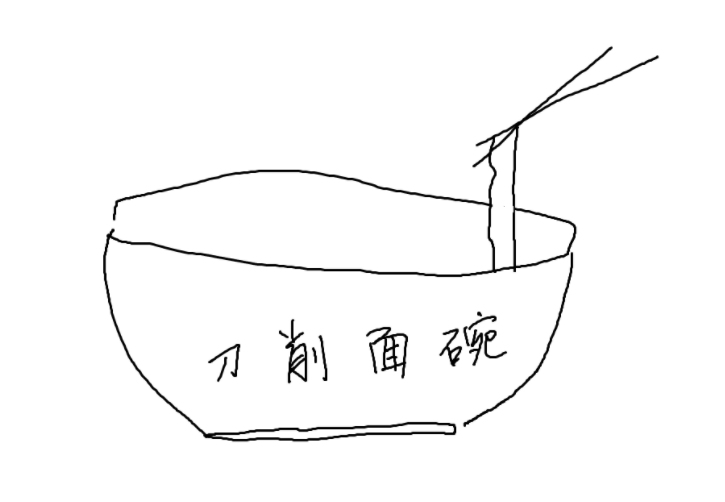
\includegraphics[width=0.7\linewidth]{img/1321screenshot002}
	\label{fig:1321screenshot002}
\end{figure}

\hfill 2024年11月13日

\end{document}
